\section{Silicon-tungsten \ecal simulation}

A standalone Geant4 package is developed to study the performance of the SiW ECAL.
Figure~\ref{fig:process} shows a flowchart of the simulation, 
reconstruction, and analysis. For the study of energy resolution and the determination of the calibration parameters, 
the input of the Geant4 simulation is simply provided by G4ParticleGun. 
For the simulation of the benchmark decay channels, 
the Gauss package (v51r2) is used to produce the input for the full simulation of the SiW ECAL. 
In the Gauss simulation the beam condition of Upgrade II is used, 
and the information of all particles before entering the calorimeter is recorded and is used later as the input of the standalone ECAL simulation. 
In this case, apart from the SiW ECAL nothing else exists in the standalone simulation.
In order to study the Bremsstrahlung effect of electrons, 
a simplified tracking system with the magnetic field before the ECAL is implemented in the simulation. 
The amount of material is around $0.6X_0$. 
In this case the input of the standalone simulation is the output of Gauss at generator level with the Upgrade II beam condition.

%%%%%%%%%%%%%%%%%%%%%%%%%%%%%%%%%%%%%%%%
\begin{figure}[hb]
  \begin{center}
    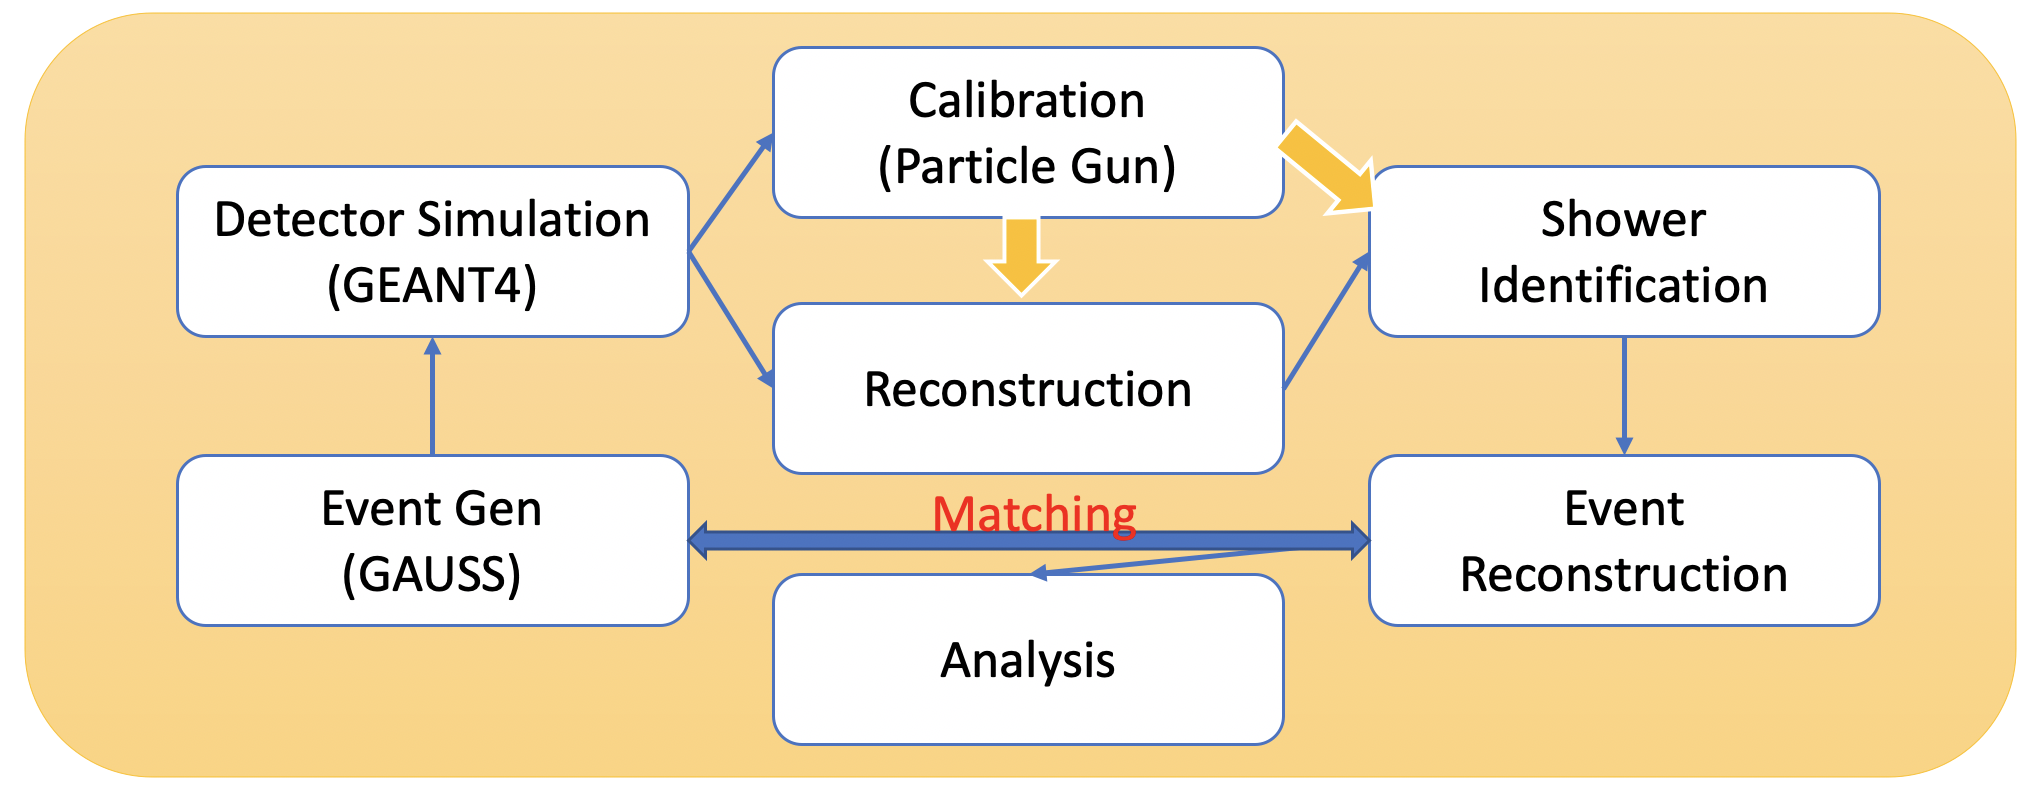
\includegraphics[width=0.95\linewidth]{Figures/06_ECAL/procedure.png}%\put(-32,133){(a)}
    \vspace*{-0.5cm}
  \end{center}
  \caption{
    %\small %captions should be a little bit smaller than main text
   The simulation process with Si-W \ecal model in \geant.
  }
  \label{fig:process}
\end{figure}
%%%%%%%%%%%%%%%%%%%%%%%%%%%%%%%%%%%%%%%%

\subsection{Simulation model in \geant}
\label{subsec:Detector}

The multi-layer SiW detector model is constructed in a standalone Geant4 framework. Details of the detector are described below.

\subsubsection{Geometry}
The default geometry of the SiW ECAL is as follows. It contains 26 layers of tungsten as the absorbers interleaved with 26 silicon layers as the active material.
The thickness of each silicon (tungsten) layer is $0.4\mm$ ($3.5\mm$).
The cell size of the Si layers is $1.01\cm\times1.01\cm$.
Figure~\ref{fig:geometrySiW} shows a side-view of the SiW ECAL with a shower of a $50\gev$ photon.
When studying the energy resolution, the thickness of each layer and the cell size are varied.
%%%%%%%%%%%%%%%%%%%%%%%%%%%%%%%%%%%%%%%%
\begin{figure}[hb]
  \begin{center}
    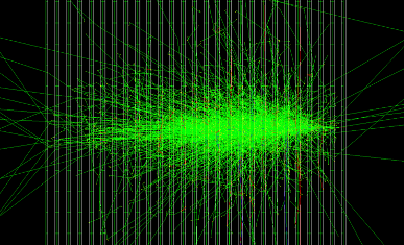
\includegraphics[width=0.6\linewidth]{Figures/06_ECAL/plotsZW/geometrySiW.pdf}%\put(-32,133){(a)}
    \vspace*{-0.5cm}
  \end{center}
  \caption{
    %\small %captions should be a little bit smaller than main text
   Geometry of the SiW ECAL used in the Geant4 simulation. Displayed is a shower of a $50\gev$ photon.
  }
  \label{fig:geometrySiW}
\end{figure}
%%%%%%%%%%%%%%%%%%%%%%%%%%%%%%%%%%%%%%%%


\subsubsection{Detection efficiency of sensors}
%The detection efficiency of $\gamma$ in each layer is studied.
%If the deposited energy in one cell is larger than $0.5\mev$, the sensor will be triggered.
%Figure~\ref{fig:detecting_eff} presents the efficiency varies with the energy and direction of the incident particle.
%It shows that the dependence of the detection efficiency on the incident angle is almost negligible, while the efficiencies for the layers in the end part of the ECAL strongly depend on the energy of the incident photon.

During the development of a shower some energies will deposit in the cells.
It is assumed here that the sensor will not be triggered if the deposited energy in one cell is less than $0.5\mev$. We define the detection efficiency of sensors as the fraction of the cells with deposited energy greater than $0.5\mev$.
One can imagine that this efficiency should be close to unit in the first stage of the shower development, while it will be small in the far-end part of the shower.
Figure~\ref{fig:detecting_eff} presents the efficiency varies with the energy and the direction of the incident particle.
It shows that the dependence of the efficiency on the incident angle is almost negligible, 
while the efficiencies for the layers in the end part of the ECAL strongly depend on the energy of the incident photon. 
One can conclude from these plots that if only a few silicon layers will be used to obtain time information of the shower, they should not be placed in the end part of the ECAL.


\begin{figure}[!htbp]
\centering
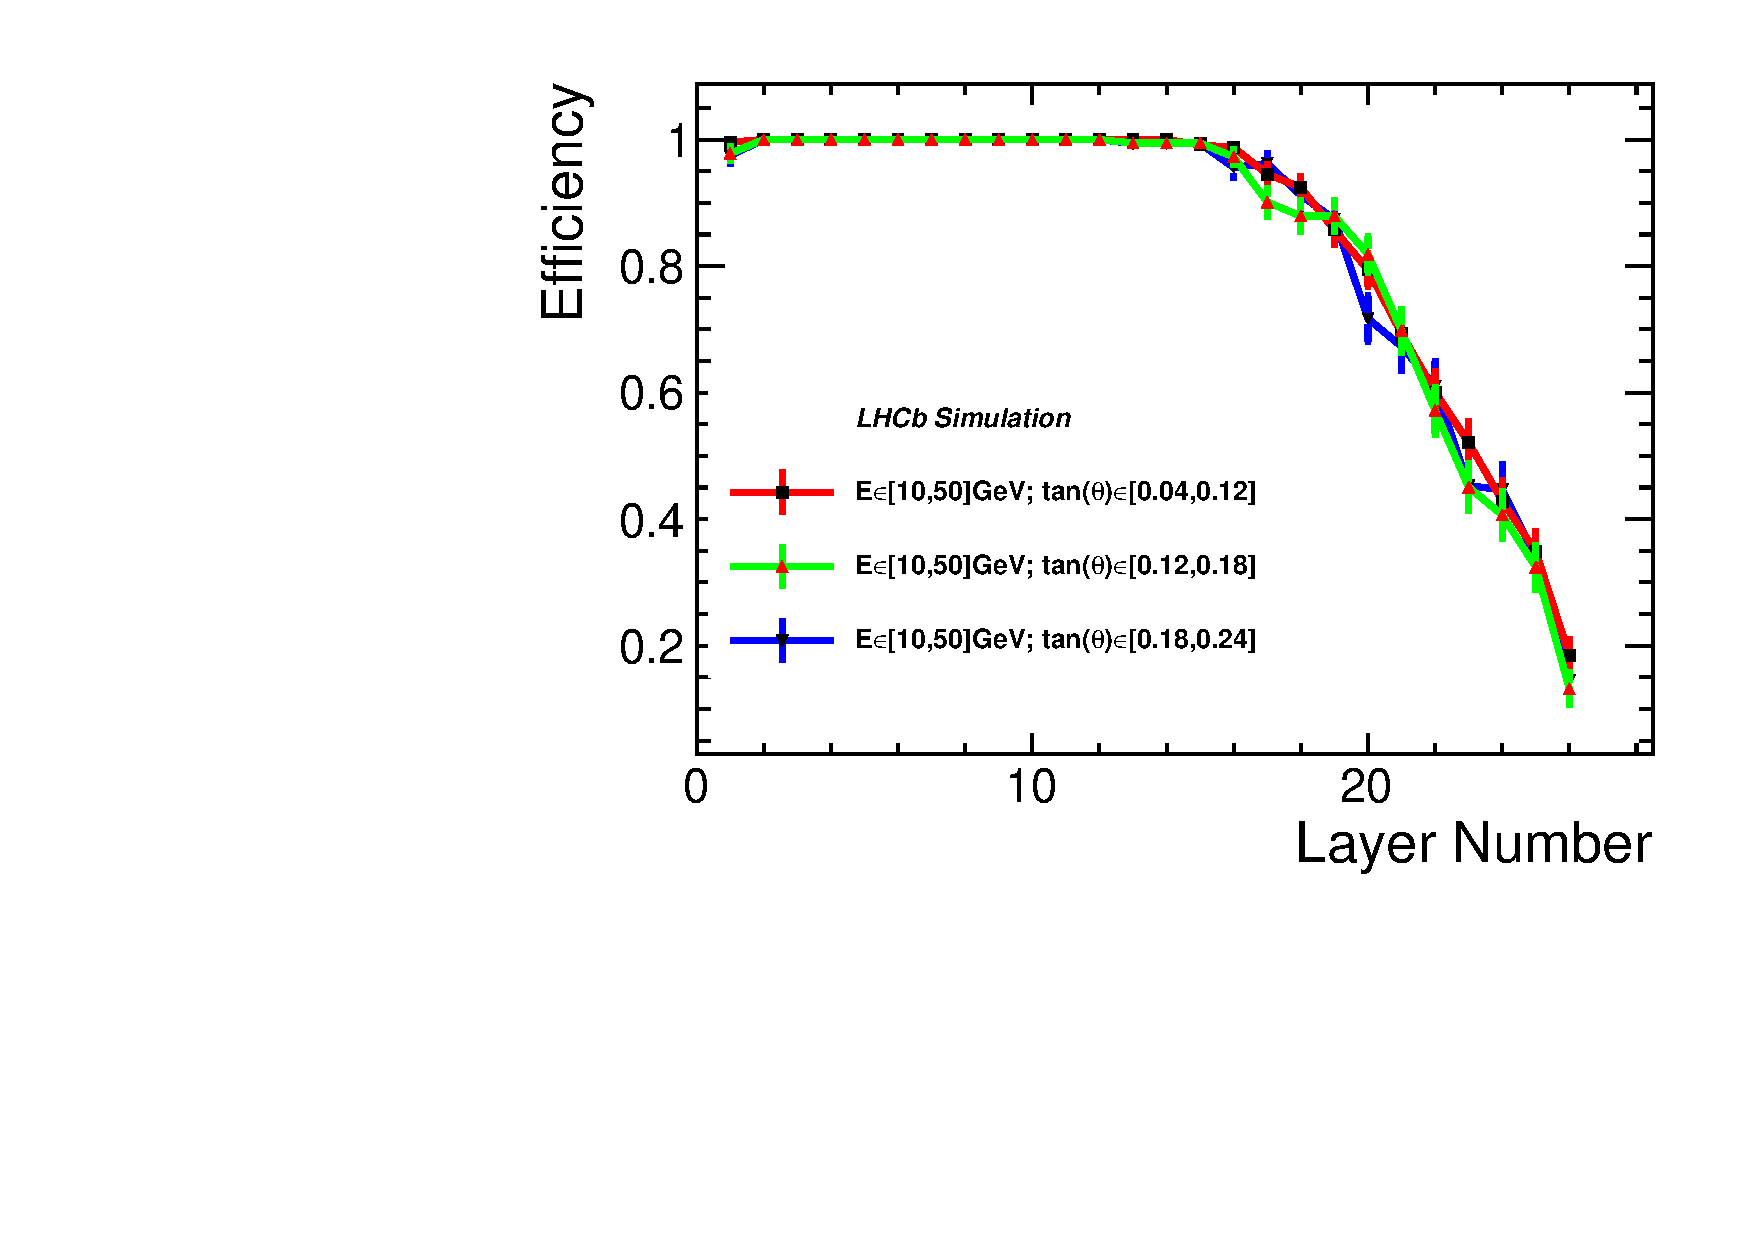
\includegraphics[width=0.48\textwidth]{Figures/06_ECAL/detecting_eff/Eff_50.pdf}
\put(-150,100) {\textrm{\small \bf(a)}}
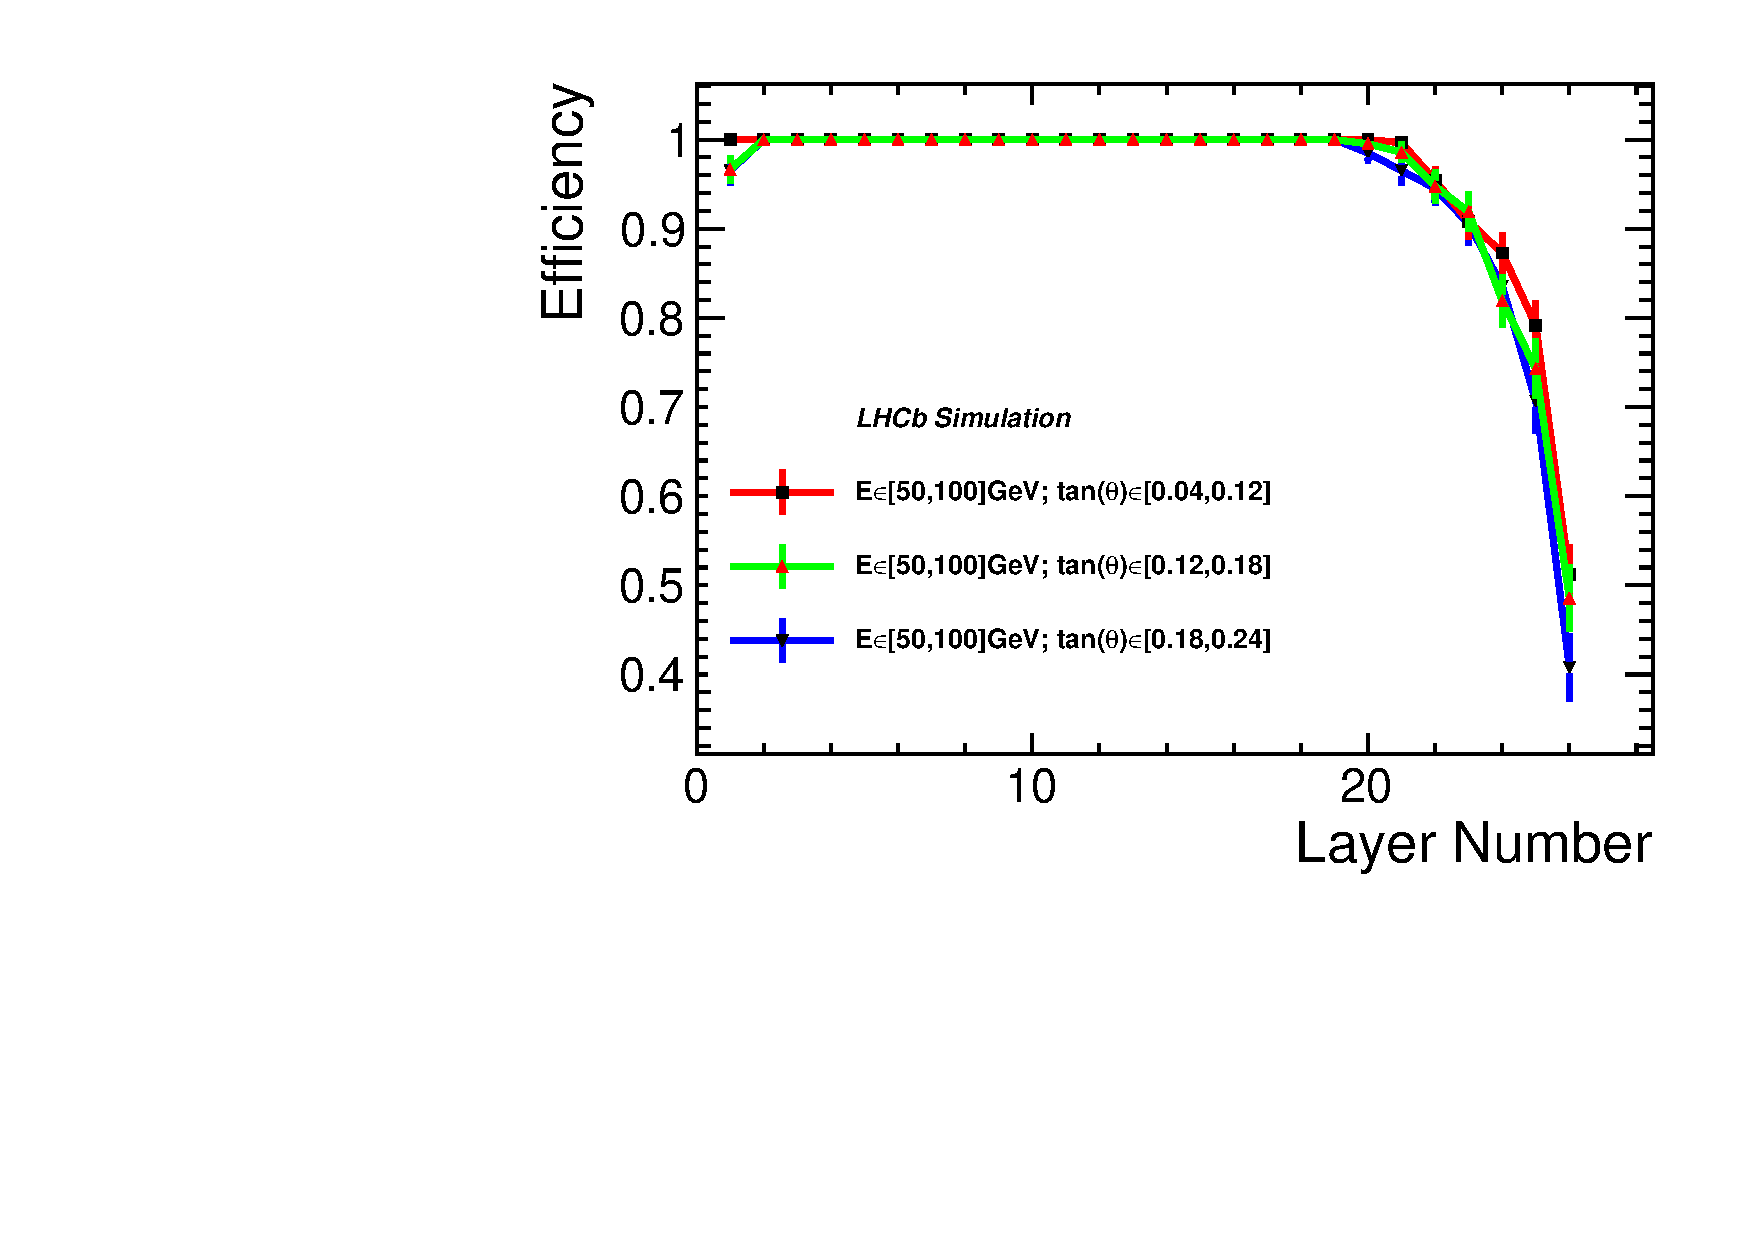
\includegraphics[width=0.48\textwidth]{Figures/06_ECAL/detecting_eff/Eff_100.pdf}
\put(-150,100) {\textrm{\small \bf(b)}}\\
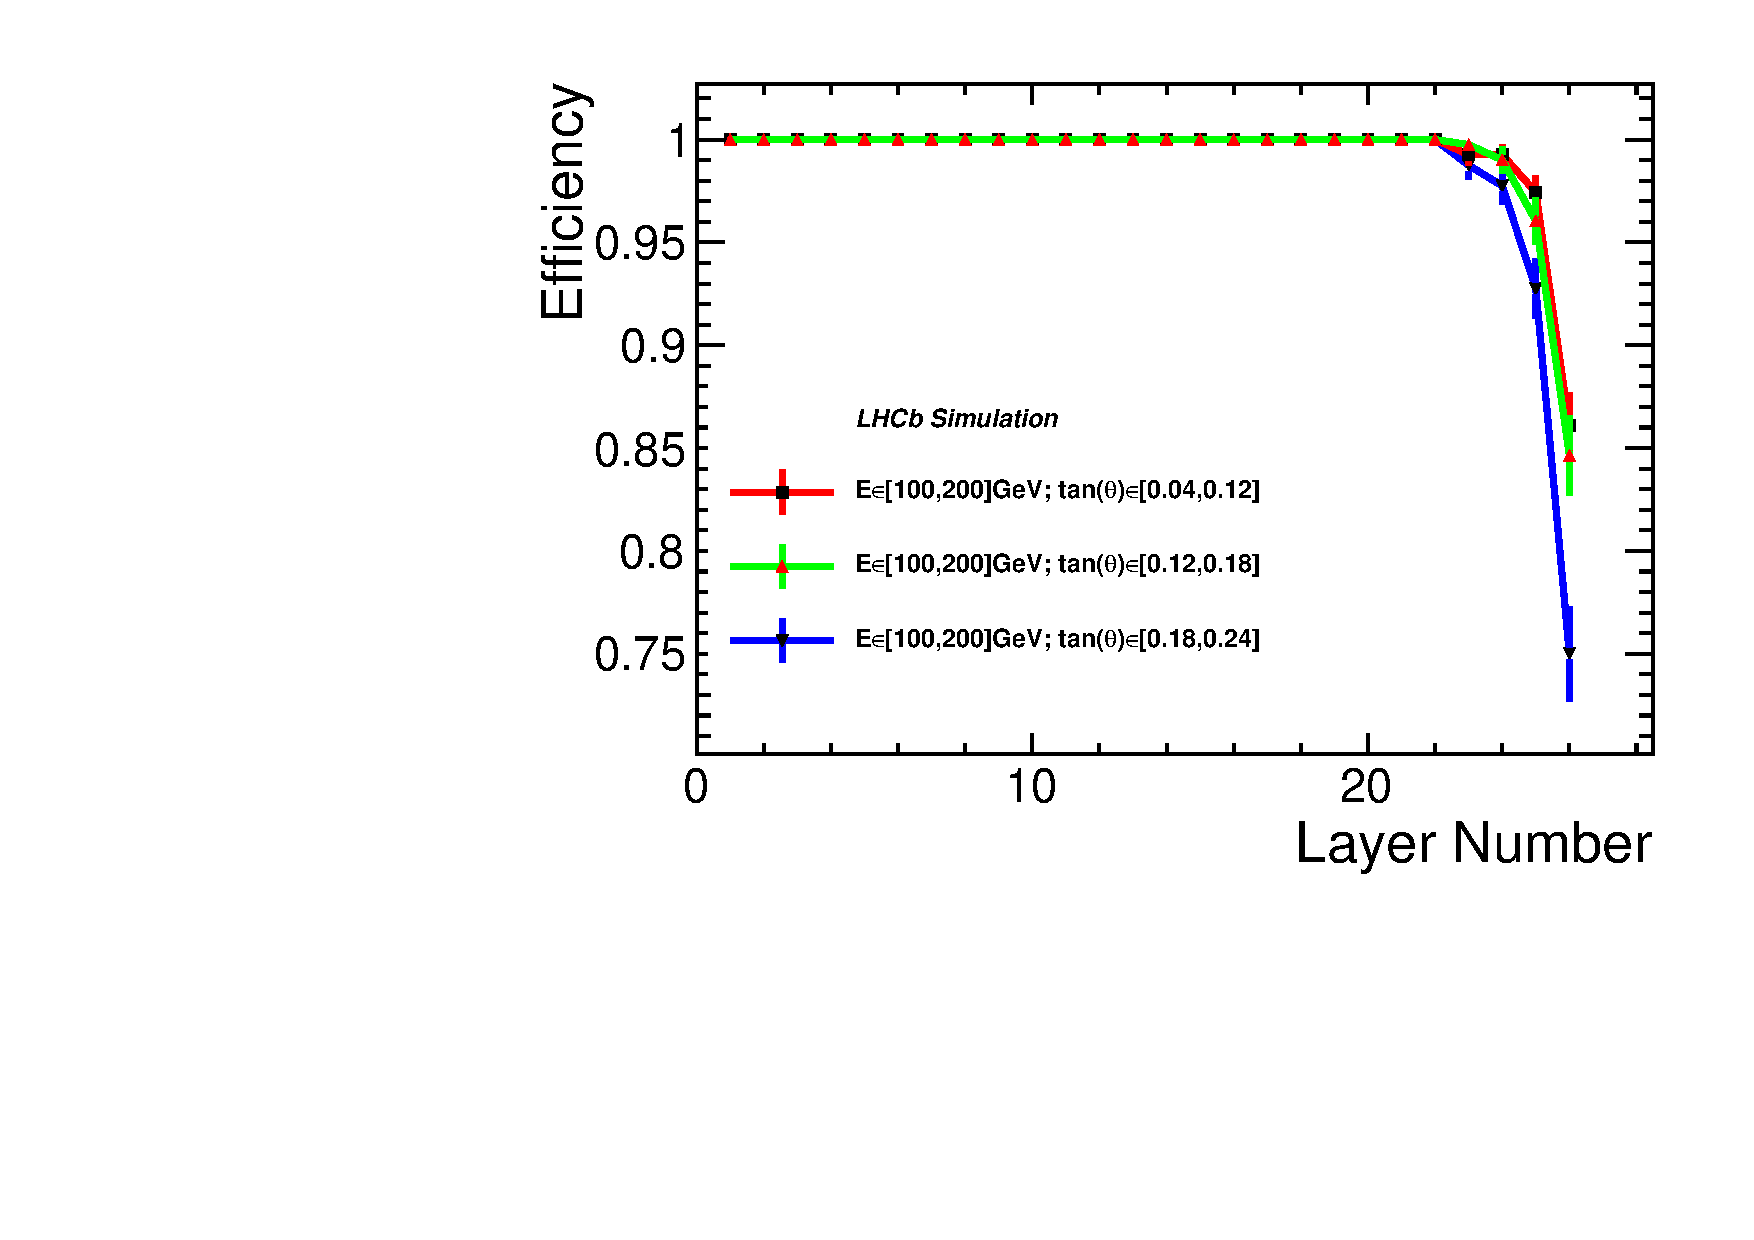
\includegraphics[width=0.48\textwidth]{Figures/06_ECAL/detecting_eff/Eff_200.pdf}
\put(-150,100) {\textrm{\small \bf(c)}}
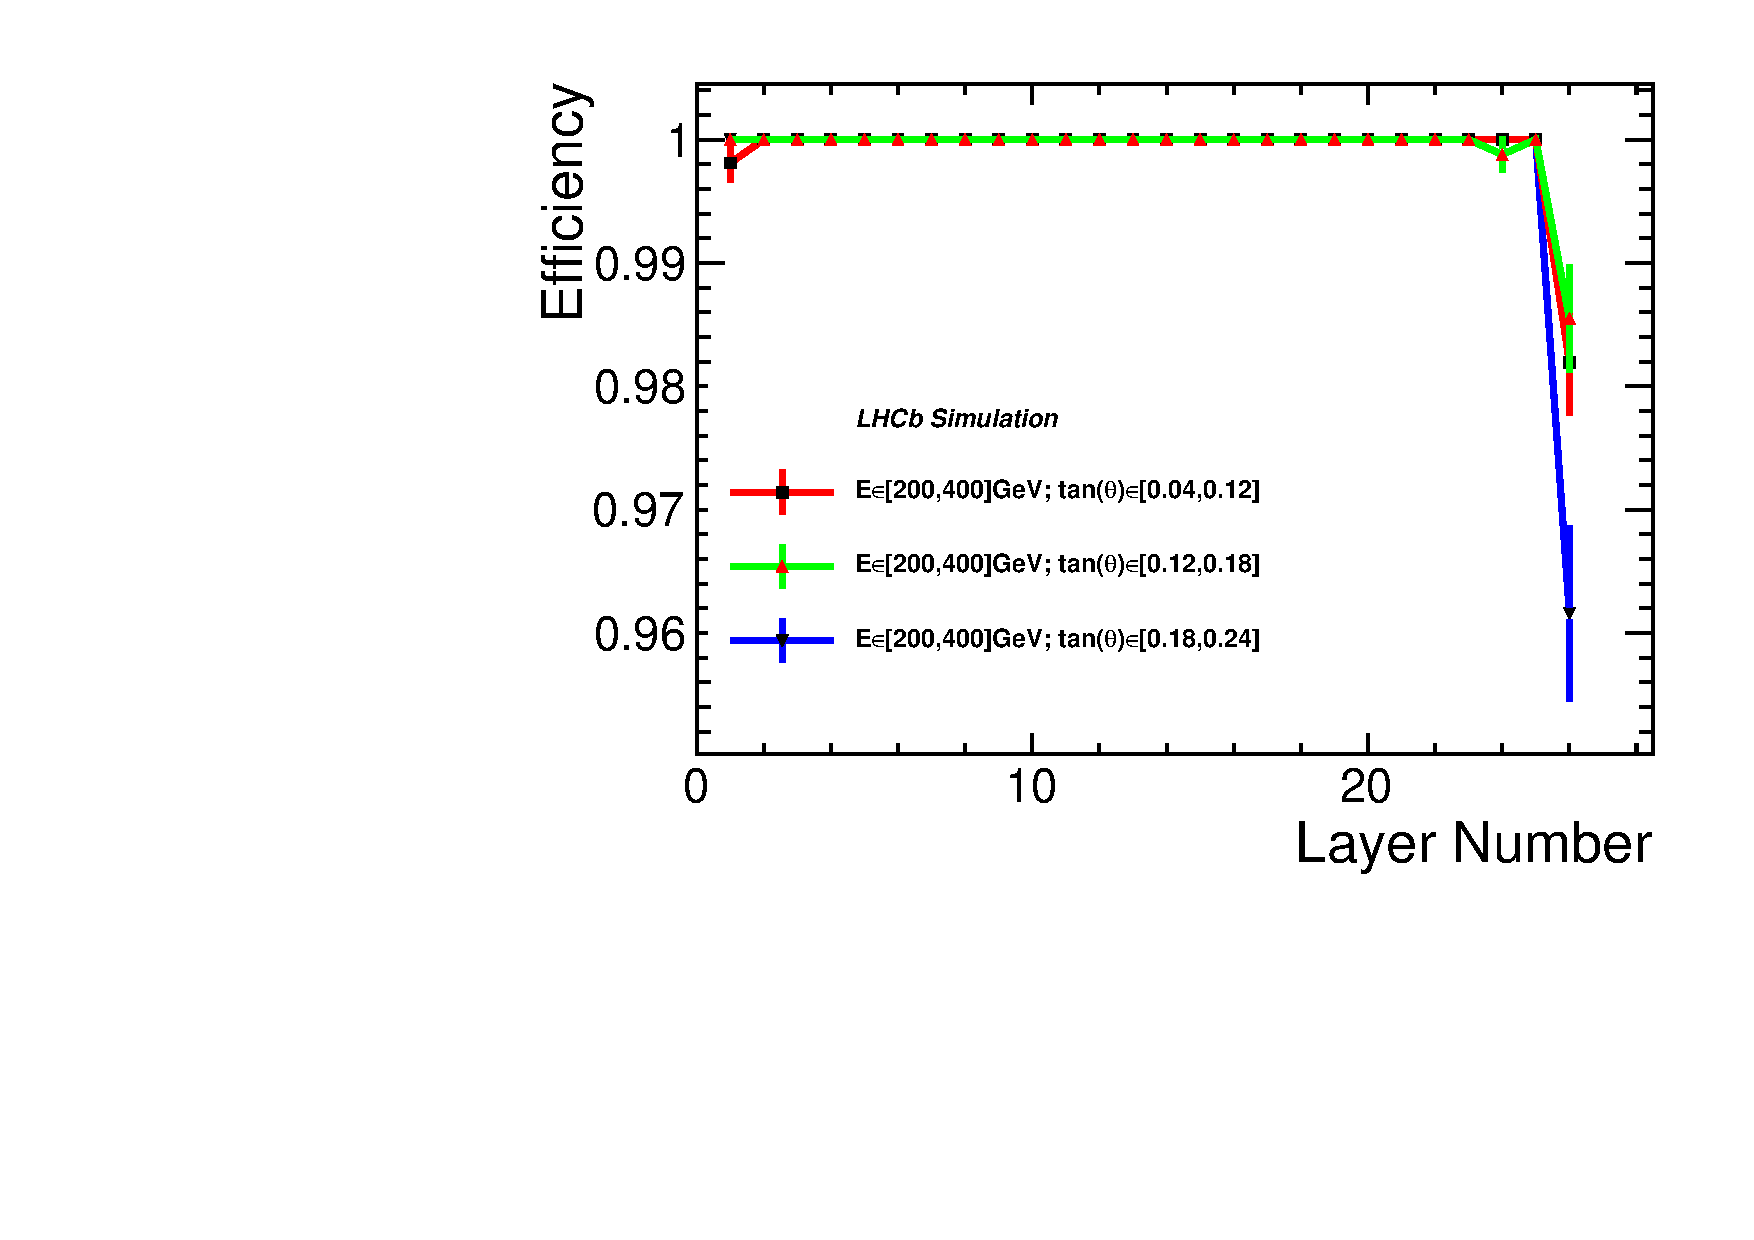
\includegraphics[width=0.48\textwidth]{Figures/06_ECAL/detecting_eff/Eff_400.pdf}
\put(-150,100) {\textrm{\small \bf(d)}}
\caption{The detection efficiency of sensors for $\gamma$ with different energy and incident directions to the \ecal plane.
}
\label{fig:detecting_eff}
\end{figure}


\subsubsection{Parameterized silicon sensor time resolution}
\label{subsubsec:para_time}

The silicon sensor provides the information of time-of-arrival (ToA).
From the CMS TDR (CERN-LHCC-2017-023) \supercite{CERN-LHCC-2017-023},
the precision of the overall timing measurement depends on the intrinsic performance of the silicon sensor, together with the preamplifier and the discriminator.
Results from the CMS beam tests \supercite{Akchurin:2018rpm} have shown that the timing resolution obtained with silicon  sensors does not vary significantly with sensor thickness when the resolution is measured as a function of the signal-to-noise ratio, $S/N$.


The timing resolution can be expressed as
\begin{equation}
\sigma_{t} = \sigma_{jitter} \oplus \sigma_{floor},
\sigma_{jitter} = \frac{A}{S/N},
\end{equation}
where
%$S/N$ is the signal-to-noise ratio,
$\sigma_{floor}$ is a constant term,
and the symbol $\oplus$ denotes quadratic summation.
The constant $A$ is fixed by the response time and noise characteristics of the sensor and the preamplifier.
According the test by CMS, the expected parameters are: $A=5\ns$, $\sigma_{floor}=20\ps$ and the $S/N$ for $MIP$ is equal to 12.
The deposited energy \mip in a $0.4\mm$-thick silicon for is around $0.16\mev$,
so the parameterized function can be written as
\begin{equation}
\sigma_{t} = \frac{5\ns}{12\times\sqrt{E/0.16}} \oplus 0.02\ns,
\end{equation}
where $E$ is the deposited energy in $\mev$. 
For safety, the parameterized time resolution used in this simulation is
\begin{equation}
\sigma_{t} = \frac{5\ns}{12\times\sqrt{E/0.2}} \oplus 0.02\ns.
\end{equation}








